\documentclass[]{article}
\usepackage{lmodern}
\usepackage{amssymb,amsmath}
\usepackage{ifxetex,ifluatex}
\usepackage{fixltx2e} % provides \textsubscript
\ifnum 0\ifxetex 1\fi\ifluatex 1\fi=0 % if pdftex
  \usepackage[T1]{fontenc}
  \usepackage[utf8]{inputenc}
\else % if luatex or xelatex
  \ifxetex
    \usepackage{mathspec}
  \else
    \usepackage{fontspec}
  \fi
  \defaultfontfeatures{Ligatures=TeX,Scale=MatchLowercase}
\fi
% use upquote if available, for straight quotes in verbatim environments
\IfFileExists{upquote.sty}{\usepackage{upquote}}{}
% use microtype if available
\IfFileExists{microtype.sty}{%
\usepackage{microtype}
\UseMicrotypeSet[protrusion]{basicmath} % disable protrusion for tt fonts
}{}
\usepackage[margin=1in]{geometry}
\usepackage{hyperref}
\hypersetup{unicode=true,
            pdftitle={methodological \& statistical issues to communicate in research proposals},
            pdfauthor={w.cools (ICDS)},
            pdfborder={0 0 0},
            breaklinks=true}
\urlstyle{same}  % don't use monospace font for urls
\usepackage{graphicx,grffile}
\makeatletter
\def\maxwidth{\ifdim\Gin@nat@width>\linewidth\linewidth\else\Gin@nat@width\fi}
\def\maxheight{\ifdim\Gin@nat@height>\textheight\textheight\else\Gin@nat@height\fi}
\makeatother
% Scale images if necessary, so that they will not overflow the page
% margins by default, and it is still possible to overwrite the defaults
% using explicit options in \includegraphics[width, height, ...]{}
\setkeys{Gin}{width=\maxwidth,height=\maxheight,keepaspectratio}
\IfFileExists{parskip.sty}{%
\usepackage{parskip}
}{% else
\setlength{\parindent}{0pt}
\setlength{\parskip}{6pt plus 2pt minus 1pt}
}
\setlength{\emergencystretch}{3em}  % prevent overfull lines
\providecommand{\tightlist}{%
  \setlength{\itemsep}{0pt}\setlength{\parskip}{0pt}}
\setcounter{secnumdepth}{0}
% Redefines (sub)paragraphs to behave more like sections
\ifx\paragraph\undefined\else
\let\oldparagraph\paragraph
\renewcommand{\paragraph}[1]{\oldparagraph{#1}\mbox{}}
\fi
\ifx\subparagraph\undefined\else
\let\oldsubparagraph\subparagraph
\renewcommand{\subparagraph}[1]{\oldsubparagraph{#1}\mbox{}}
\fi

%%% Use protect on footnotes to avoid problems with footnotes in titles
\let\rmarkdownfootnote\footnote%
\def\footnote{\protect\rmarkdownfootnote}

%%% Change title format to be more compact
\usepackage{titling}

% Create subtitle command for use in maketitle
\newcommand{\subtitle}[1]{
  \posttitle{
    \begin{center}\large#1\end{center}
    }
}

\setlength{\droptitle}{-2em}

  \title{methodological \& statistical issues\\
to communicate in research proposals}
    \pretitle{\vspace{\droptitle}\centering\huge}
  \posttitle{\par}
    \author{w.cools (ICDS)}
    \preauthor{\centering\large\emph}
  \postauthor{\par}
      \predate{\centering\large\emph}
  \postdate{\par}
    \date{\today}

\usepackage{titling}
\usepackage[export]{adjustbox}
\pretitle{%
  \begin{center}
  \LARGE
  \begin{figure}[!h]
  	\begin{minipage}{4cm}
  		
\includegraphics[width=4cm,height=1cm,left]{umc.png}\\[\bigskipamount]
  	\end{minipage}
  	\hfill
  	\begin{minipage}{4cm}	
  		
\includegraphics[width=4cm,height=1cm,right]{icds.png}\\[\bigskipamount]
  	\end{minipage}
  \end{figure}
}
\posttitle{\end{center}
}

\begin{document}
\maketitle

\subsubsection{Why and What}\label{why-and-what}

\begin{itemize}
\tightlist
\item
  convince referees (and yourself) that your study will be successful,
  effective and efficient
\item
  beware that some referees are statisticians, they do not understand
  your area of expertise
\item
  to help write proposals statistician proof, a document was created
  (pdf/html): `methodological \& statistical issues to communicate in
  research proposals' which will be updated and refined
\item
  disclaimer: no full coverage is pretended, books have been written on
  the various topics included in current draftthe drafts also reflects
  our own view, not necessarily the view of all possible referees you
  come across, so, please use this draft only for guidance and not as an
  argument or proof of any kind.
\end{itemize}

\subsection{Key Ingredients}\label{key-ingredients}

\begin{itemize}
\tightlist
\item
  there are two key ingredients in terms of methodology

  \begin{itemize}
  \tightlist
  \item
    you should specify what is the aim of your study
  \item
    you should introduce how you study is designed to achieve that aim
  \end{itemize}
\item
  aim and design should match, often statistics is required for the
  match
\end{itemize}

\begin{figure}[htbp]
\centering
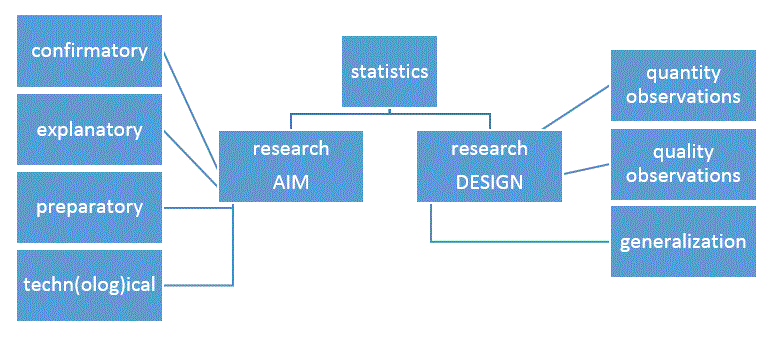
\includegraphics{graph.png}
\caption{outline: key ingredients and main components}
\end{figure}

\begin{center}\rule{0.5\linewidth}{\linethickness}\end{center}

\subsection{Research Aim}\label{research-aim}

\begin{itemize}
\tightlist
\item
  the research aim typically is a question that your research can
  provide answers for, note that questions are not stories, nor a
  description of results
\item
  when specifying the research questions, be specific, so if the
  questions are put in general terms also operationalize them
\item
  focus, even though your study will be able to provide many interesting
  findings, typically the study is designed with a few main questions of
  primary interest
\item
  for the main questions of interest, specify what the results should be
  at a minimum to make the study successful, this is used to evaluate
  whether the study is interesting, and whether the aim can be achieved
\item
  for the remainder, explain all the other possible interesting findings
  that may and might show, findings that are not required to make the
  study a success but will nevertheless potentially make the study more
  interesting 
\item
  several types of aim can be distinguished, and will be discussed in
  current draft

  \begin{itemize}
  \tightlist
  \item
    confirmatory / exploratory / preparatory / techn(olog)ical
  \item
    quantitative / qualitative
  \item
    inferential / descriptive
  \end{itemize}
\end{itemize}

\subsubsection{Confirmatory (purpose A)}\label{confirmatory-purpose-a}

\begin{itemize}
\tightlist
\item
  goal:: confirm an expected difference, relation, \ldots{} maybe the
  aim is to establish a difference or a pre-specified certainty on a
  parameter estimate
\item
  focus:: statistical test or accurate parameter estimate
\item
  requirement::

  \begin{itemize}
  \tightlist
  \item
    sample size calculation, if not enough information is obtained to
    make the confirmation the study failed

    \begin{itemize}
    \tightlist
    \item
      absence of proof is not proof of absence
    \item
      non-significant results can be due to the lack of effect or the
      lack of power
    \end{itemize}
  \item
    discuss costs and availability of observations in light of the
    required sample size, note that interim analysis may be interesting
    but require a more complicated sample size estimation
  \item
    the link between the research design and especially the primary aim
    is important to specify, which should link up nicely with the
    statistical analysis plan
  \end{itemize}
\item
  minimum:: a study would be successful if it is considered interesting
  by expert peers and if the effect is significant or accurate enough 
\item
  a special note is due on statistical testing, the aim is not always to
  establish a difference or relation, sometimes it involves

  \begin{itemize}
  \tightlist
  \item
    superiority, which requires a sample size to show that some set of
    observations is not worse, with a pre-specified margin
  \item
    non-equivalence, to show similarity, which requires a sample size
    for two tests, one to show that the effect can not be smaller than
    the pre-specified lower margin of tolerance and one that it can not
    be bigger than the upper margin of tolerance
  \end{itemize}
\end{itemize}

\subsubsection{Exploratory (purpose B)}\label{exploratory-purpose-b}

\begin{itemize}
\tightlist
\item
  goal:: to explore, there is no clear idea on what the effect should be
  and what the population variance of the measurement would be
\item
  while not easy to justify, exploratory studies are quite common

  \begin{itemize}
  \tightlist
  \item
    focus A:: the interest could be merely a data description and/or
    parameter estimation, where the results would be interesting
    whatever they are

    \begin{itemize}
    \tightlist
    \item
      while testing/accuracy is not the primary aim, it could be
      secondary in a sense that significance/accuracy is not guaranteed
      in advance
    \end{itemize}
  \item
    focus B:: most qualitative understanding is exploratory
  \item
    focus C:: various statistical procedures are not (yet) developed
    enough to provide clear aims for, like hierarchical clustering,
    \ldots{}, are the ever more popular predictive modeling that is
    evaluated using cross-validation instead of significance testing
  \end{itemize}
\item
  requirement::

  \begin{itemize}
  \tightlist
  \item
    because it is hard or impossible to justify a study based on
    statistics, the need/importance of extracted information should be
    made clear on substantive grounds, without reference to statistical
    tests
  \item
    a sample size -justification- would argue for a balance between
    information and cost
  \item
    the link between the research design and the most important
    information of interest is still of interest, but various hypotheses
    are now typically of interest, all requiring a statistical plan
  \end{itemize}
\item
  minimum:: the justification for exploratory studies could be many
  things, as long as you can sufficiently argue its merit, again,
  without any reference to significance/accuracy.
\end{itemize}

\subsubsection{Preparatory (purpose C)}\label{preparatory-purpose-c}

\begin{itemize}
\tightlist
\item
  goal:: while very similar to exploratory studies, preparatory studies
  (my own label) prepare or justify a future study, the results are not
  by themselves of interest
\item
  focus: tyically this type of study implies a small scale set-up to
  show the potential and/or detect issues, again, not set up to
  establish effects

  \begin{itemize}
  \tightlist
  \item
    phase I and II clinical designs

    \begin{itemize}
    \tightlist
    \item
      such designs are required to decide on whether further studies
      would be of high enough potential while accounting for the costs
      involved, it requires decision criteria to proceed or not
    \end{itemize}
  \item
    pilot study, which serve to prepare to implement a future study

    \begin{itemize}
    \tightlist
    \item
      no statistical testing is implied, that is for the actual study
    \item
      not in itself of interest, therefore not intended for publication
    \item
      could be (partially) qualitative, in fact, everything goes if it
      provides the required information, it could even be simply
      monitoring (part of) the intended procedures (not a mini-copy)
    \end{itemize}
  \end{itemize}
\item
  requirement::

  \begin{itemize}
  \tightlist
  \item
    it should be clear that the required information will be obtained,
    but also the future study itself should be made clear
  \item
    a minimal cost to get a rough idea should suffice, for example, with
    animal experiments this typically results in 3 animals per condition
    which allow for an estimate of variance
  \end{itemize}
\item
  minimum: at least the information required for the future study should
  come out, but there are no strict rules otherwise
\end{itemize}

\subsubsection{Techn(olog)ical advancements (purpose
D)}\label{technological-advancements-purpose-d}

\begin{itemize}
\tightlist
\item
  goal:: to design, engineer, create, \ldots{} not all studies are set
  up to extract information from the outside world
\item
  focus:: when not focused on information, rarely there is any
  statistics involved
\item
  requirement:: there are therefore no requirements in terms of
  methodology or statistics, the justification should be based on the
  expected contribution to research versus the cost

  \begin{itemize}
  \tightlist
  \item
    proof of concept: feasibility
  \item
    proof of principle: functionality
  \item
    development application
  \end{itemize}
\item
  minimum:: the merit should be shown, and at least a particular state
  of advancement should be expected
\end{itemize}

\subsubsection{Additional distinctions in
aim}\label{additional-distinctions-in-aim}

\begin{itemize}
\tightlist
\item
  Quantitative versus Qualitative

  \begin{itemize}
  \tightlist
  \item
    quantitative research focuses on quantifiable empirical aspects, and
    typically in doing so reduces the complexity in order to make use of
    visualization and statistics to summarize and generalize, this type
    of research can be both descriptive and/or inferential
  \item
    qualitative research focuses on understanding, especially with focus
    on reasons, opinions, motivations, \ldots{} trying to embrace the
    complexity involved, but in doing so limiting the study to
    descriptive research that is at most hypothesis generating 
  \end{itemize}
\item
  Descriptive versus Inferential

  \begin{itemize}
  \tightlist
  \item
    inferential research is about the population, based on a sample,
    which implies generalization and therefore (ideally) representative
    samples for which it uses uncertainty
  \item
    descriptive research is about the sample and does not go beyond the
    observed data, which is why data are presented as is without
    reference to uncertainty nor p-values 
  \end{itemize}
\item
  while used here to show distinctions, they can be combined into one
  study
\end{itemize}

\begin{center}\rule{0.5\linewidth}{\linethickness}\end{center}

\subsection{Research Design}\label{research-design}

\begin{itemize}
\tightlist
\item
  the research design is strategy to achieve the research aim

  \begin{itemize}
  \tightlist
  \item
    it can include aspects related to data collection, measurement, and
    even the intended analyses
  \item
    in a strict sense, the design specifies how (potential) observations
    are related which influences the information that can be extracted
    \\
  \end{itemize}
\item
  there is a popular saying: garbage in\ldots{} garbage out !

  \begin{itemize}
  \tightlist
  \item
    a poor design makes a study inefficient at best, or even completely
    invalid at worst
  \item
    note that statistics can not solve design problems\\
  \end{itemize}
\item
  there are three types of design specification, four if you count
  statistics

  \begin{itemize}
  \tightlist
  \item
    a design is determined by the quantity of observations, the sample
    size, which should be sufficient
  \item
    designs can differ in quality, dependent on

    \begin{itemize}
    \tightlist
    \item
      conditions and method of observation
    \end{itemize}
  \item
    generalization to the population is dependent on

    \begin{itemize}
    \tightlist
    \item
      selection of research units and missing observations
    \end{itemize}
  \item
    allowing appropriate statistical analysis
  \end{itemize}
\end{itemize}

\subsubsection{Quantity of Observations}\label{quantity-of-observations}

\begin{itemize}
\tightlist
\item
  observations should provide information on the questions of interest

  \begin{itemize}
  \tightlist
  \item
    this implies that more observations are more informative
  \item
    but, observations come with a cost, so there is a reason not to make
    too many
  \item
    costs can exist in terms of time, money, risk, \ldots{} 
  \end{itemize}
\item
  when confirmatory studies are of interest, sample size -calculation-
  should be performed and communicated

  \begin{itemize}
  \tightlist
  \item
    specify the statistical test in focus, this should reflect the
    minimal result for the main hypothesisdo not assume that the test is
    clear from the context
  \item
    determine the effect size aimed for, and give good enough reasons
    for it, for both the effect and the uncertainty

    \begin{itemize}
    \tightlist
    \item
      effect: know what you want to find, ideally specified
      substantively but otherwise referring to common practice / earlier
      research (effect size is signal)
    \item
      uncertainty: understand the population variance of your
      measurement, ideally based on earlier data/research or pilot
    \item
      use rules of thumb when all reasoning fails, only
    \end{itemize}
  \item
    operational characteristics (type I error \(\alpha\) and type II
    error \(\beta\)), typically with power ranging between .8 and .9,
    note that the two types of errors are related, decreasing one would
    increase the other keeping the sample size constant note that with
    \(\alpha\) .05 and power .8, the type I error \(\alpha\) is
    considered 4 times more severe than the type II error \(\beta\) 
  \item
    there are two issues worth mentioning:

    \begin{itemize}
    \tightlist
    \item
      sample size calculation is relevant for the primary research
      questions, if there are multiple that are related the highest
      value is usually considered
    \item
      only use sample size calculation, or power analysis, for future
      studies, never to justify data can be analyzed already (not
      retrospective)
    \end{itemize}
  \end{itemize}
\end{itemize}

\subsubsection{Quality of Observations}\label{quality-of-observations}

\begin{itemize}
\tightlist
\item
  the quality of observations depends on conditions under which they
  were observed and the method used for making the observation 
\item
  general idea is to isolate the effect, either by avoiding or by
  measuring the unwanted influences on the observations
\item
  a general principle is to try and

  \begin{itemize}
  \tightlist
  \item
    control confounding variables (influence not in the model)
  \item
    maximize systematic variability (explained variance)
  \item
    minimize non-systematic variability (unexplained variance) \\
  \end{itemize}
\item
  exercising that principle often implies control, at least to some
  extent

  \begin{itemize}
  \tightlist
  \item
    an experimental study exerts control, by definition, therefore it
    typically offers more quality in terms of observations

    \begin{itemize}
    \tightlist
    \item
      necessary condition for causal conclusions
    \end{itemize}
  \item
    observational study does not exert control, therefore often the
    quantity has to be increased rather than the quality

    \begin{itemize}
    \tightlist
    \item
      naturalistic, survey, \ldots{} most retrospective
    \end{itemize}
  \end{itemize}
\end{itemize}

\subsubsection{Quality of Observations ---
Confounders}\label{quality-of-observations-confounders}

\begin{itemize}
\tightlist
\item
  control on confounding variables, to avoid differential influence on
  the observations from unknown sources

  \begin{itemize}
  \tightlist
  \item
    randomization (large enough sample size), the most often used method
    to balance out different sources of confounding
  \item
    repeated measures, to keep various sources stable and measure their
    variance
  \item
    blocking, to keep various sources stable and measure their variance
  \item
    matching, to keep groups comparable
  \item
    cross-over designs, to create within unit comparisons and allow
    estimation of order effects
  \item
    (double-) blinding, to avoid unwanted influence from knowing the
    goal of the study
  \item
    and more \ldots{} 
  \end{itemize}
\item
  typically, upgrading the design makes it more interesting, but it does
  also complicate the statistical analysis

  \begin{itemize}
  \tightlist
  \item
    the correlational structure implied by the design has to be
    accounted for, this would often require mixed models
  \end{itemize}
\end{itemize}

\subsubsection{Quality of Observations --- (Non-) Systematic
Variability}\label{quality-of-observations-non--systematic-variability}

\begin{itemize}
\tightlist
\item
  to maximize systematic variability can be considered from two
  perspectives

  \begin{itemize}
  \tightlist
  \item
    use proper explanatory variables, in other words make sure the
    relevant explaining variables are registered properly
  \item
    use maximally differentiating conditions, in other words make sure
    that the conditions within explaining variables are selected to
    maximize the informational potential

    \begin{itemize}
    \tightlist
    \item
      beware: if focusing on the extremes, there is a threat of
      introducing artifacts
    \item
      beware: if the evolution in between also is important, some
      conditions should be set up to make observations there as well \\
    \end{itemize}
  \end{itemize}
\item
  minimize non-systematic variability, avoid everything you know nothing
  about as good as possible

  \begin{itemize}
  \tightlist
  \item
    maximize systematic variability, in other words, try to explain as
    much as possible
  \item
    use proper measurement tools

    \begin{itemize}
    \tightlist
    \item
      your measurement should be of high reliability / precision, if not
      this would increase the non-systematic variability
    \item
      to get sense on the reliability, different measurement tools can
      be combined and analysed
    \end{itemize}
  \item
    use categories when necessary only, continuous if possible, to allow
    an analysis on the finest grid possible and/or valid
  \end{itemize}
\end{itemize}

\subsubsection{Generalizability}\label{generalizability}

\begin{itemize}
\tightlist
\item
  generalization (inference) is dependent on successful sampling, in
  theory you can only draw conclusions on the population you have
  observed by sample

  \begin{itemize}
  \tightlist
  \item
    the method of sampling thus plays an important rule

    \begin{itemize}
    \tightlist
    \item
      probabilistic (sampling: random, stratified, multi-stage,
      \ldots{}.), necessary for conclusive, unbiased, objective
      inferences
    \item
      non-probabilistic (sampling: diversity, expert, \ldots{}.),
      potentially biasing, more subjective, and best used only
      explorative
    \end{itemize}
  \item
    missing data can have an effect on the generalizability depending on
    the mechanism of missingness

    \begin{itemize}
    \tightlist
    \item
      missing (completely) at random would result in efficiency loss
      primarily, missing not at random is a problem because bias is
      introduced

      \begin{itemize}
      \tightlist
      \item
        avoid missing data, explain how
      \item
        remediate, explain how
      \end{itemize}
    \end{itemize}
  \end{itemize}
\end{itemize}

\subsubsection{Small Example}\label{small-example}

The aim is to show that the proposed treatment is an improvement over
the current standard method.

Participants are randomized into two groups, treatment and control. The
control group is given a dummy treatment. A post experiment survey
addresses whether participants were aware about dummy treatment. Each
participant is measured once, immediately after the (dummy) treatment
was administered which results in one score per patient, continuous on a
0-10 scale. A t-test for independent means is used to evaluate whether
the scores in the treatment group are higher than those in the control
group.

A sample size was derived for the t-test to detect a minimal difference
of 2 in favor of the treatment, which was decided upon by our expert
panel. In literature, the standard method is indicated to have a
population standard deviation of about 4. Because no information is
available on the new treatment it is assumed that the same population
standard deviation applies. This leads to a sample size of 51 patients
in each of both groups, required for a one-sided test, type I error of
.05 and power of .8. Earlier experiments showed a drop-out of about
10\%, so 51/9*10 \textless{} 57 patients are included per group.

\subsection{Statistics}\label{statistics}

\begin{itemize}
\tightlist
\item
  statistics are used to extract information from the observations,
  which can be done in various ways

  \begin{itemize}
  \tightlist
  \item
    statistical tests evaluate whether effects exist (significance)
  \item
    statistical estimation evaluate the size of the confidence interval,
    by estimating uncertainty
  \item
    prediction of individual observations would show which conditions
    are of interest, using cross validation 
  \end{itemize}
\item
  introduce the statistics that are planned, with a focus on the main
  aims and a sketch of the secondary ones 
\item
  the statistics often is the bridge between research design and
  research aim, they should be in agreementhighlight how the statistical
  analysis is able to answer your research question, with reference to p
  values, confidence intervals, predictions, \ldots{} or whatever is
  necessary given your aim
\item
  give a rough idea about the analyses that will be used to answer the
  questions that are less in focus but that may still be of interest
\item
  reflect on the type of data, to foresee the possible challenges they
  may bring to the analysis and maybe even think on how to avoid it
  using appropriate designsthe expected data file should be given some
  serious thought in order to avoid unpleasant surprises, do not just
  observe and then fail to analyse 
\item
  note that sample size calculations are not a part of the statistical
  plan
\end{itemize}

\subsection{Practical Suggestions}\label{practical-suggestions}

\begin{itemize}
\tightlist
\item
  isolate methodological and statistical issues from substantive
  reasoning
\item
  use consistent labeling
\item
  visualize wherever possible

  \begin{itemize}
  \tightlist
  \item
    data collection process (time-line)
  \item
    categories of observations and their relation
  \item
    show design with tableslist all conditions between (rows) and within
    (columns)
  \end{itemize}
\end{itemize}

\begin{figure}[htbp]
\centering
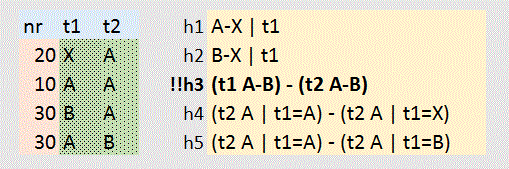
\includegraphics{conds.png}
\caption{example for specifying conditions}
\end{figure}

\subsection{Conclusion}\label{conclusion}

\begin{itemize}
\tightlist
\item
  many methodological and statistical issues, some may be relevant
\item
  convince yourself that your study is appropriate
\item
  be clear on your aim and how to be successful (research design)
\item
  convince the committee that your study is appropriate
\item
  for support, maybe turn to ICDS
\end{itemize}

\begin{figure}[htbp]
\centering
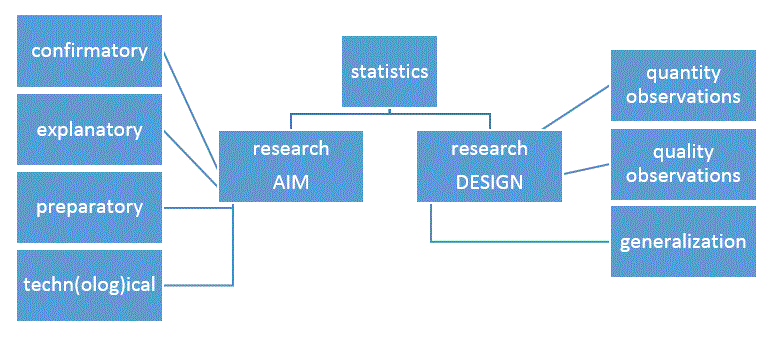
\includegraphics[width=0.70000\textwidth]{graph.png}
\caption{}
\end{figure}

\begin{center}\rule{0.5\linewidth}{\linethickness}\end{center}

\begin{center}\rule{0.5\linewidth}{\linethickness}\end{center}

\subsection{\texorpdfstring{\protect
\includegraphics[width=0.10000\textwidth]{icds.png}
Interfaculty Center Data processing \&
Statistics}{ Interfaculty Center Data processing \& Statistics}}\label{interfaculty-center-data-processing-statistics}

Methodological and statistical support to help make a difference

\begin{itemize}
\item
  ICDS provides complementary support in methodology and statistics to
  our research community, for both individual researchers and research
  groups, in order to get the best out of them
\item
  ICDS aims to address all questions related to quantitative research,
  and to further enhance the quality of both the research and how it is
  communicated
\end{itemize}

website: \url{https://www.icds.be/} includes information on who we
serve, and how booking: \url{https://www.icds.be/consulting.php} for
individual consultations


\end{document}
